\chapter{Phương pháp nghiên cứu}
Trong nghiên cứu này, tôi đã trích xuất các đặc trưng dựa trên thời gian, dựa trên lịch học tập, vị trí, và di chuyển. Đầu tiên, các đặc trưng dựa trên thời gian, bao gồm ngày trong tuần và tuần, được trích xuất. Tiếp theo, tín hiệu GPS của người tham gia sẽ được mã hóa thành tên và loại địa điểm, và được nhóm thành các loại số liệu dựa trên vị trí dựa trên loại và tên của địa điểm đã được trích xuất trước đó. Tiếp theo, tôi sử dụng lịch học tập của sinh viên để tìm lịch trình các lớp học trong một ngày (lịch học). Sau đó, việc ước tính số buổi học bị học sinh bỏ sẽ được thực hiện bằng cách so sánh lịch học với vị trí của sinh viên. Tiếp theo, các thời hạn nộp bài học tập và thời hạn nộp bài học tập sắp tới của sinh viên được trích xuất. Sau đó, bộ dữ liệu được chia thành tập huấn luyện và tập kiểm thử theo tỷ lệ 7:3. Sau đó, tôi đã huấn luyện và kiểm tra các mô hình học máy đã chọn (Random Forest, XGBoost, SVM). Cuối cùng, SHAP được áp dụng để hiểu tác động của từng yếu tố lên quyết định của mô hình.

\begin{figure}
    \centering
    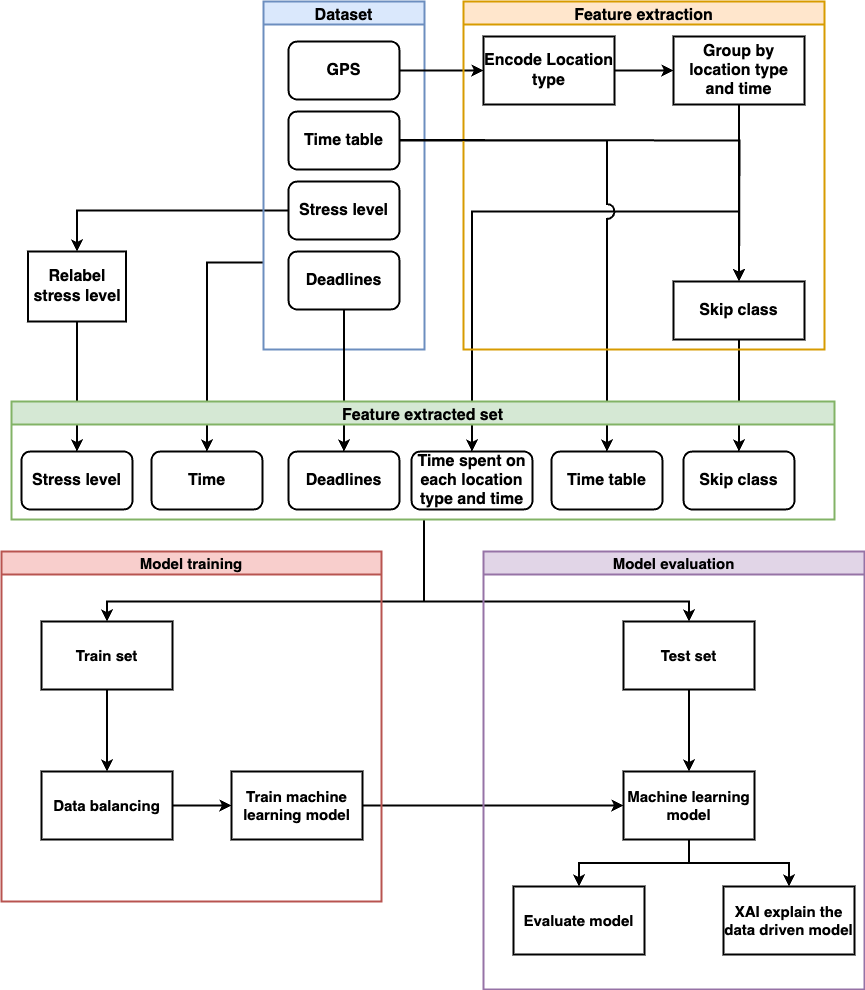
\includegraphics[width=\linewidth]{Images/pipeline_stress.drawio.png}
    \caption{Lưu đồ phương pháp nghiên cứu}
    \label{fig:enter-label}
\end{figure}

\section{Bộ dữ liệu}
Trong nghiên cứu này, bộ dữ liệu StudentLife \cite{student_life} đã được sử dụng để khai thác đặc trưng và phân tích thông tin. Bộ dữ liệu này, được thu thập vào năm 2014, đã sử dụng một ứng dụng Android để theo dõi liên tục nhiều luồng dữ liệu khác nhau bao gồm GPS, nhật ký cuộc trò chuyện, mô hình giấc ngủ và hoạt động ăn uống, bên cạnh việc theo dõi tình trạng sức khỏe tâm thần, sự tham gia lớp học, tâm trạng và hoạt động thể chất của những người tham gia tình nguyện. Bộ dữ liệu bao gồm thông tin từ 48 sinh viên trong một học kỳ 10 tuần tại Đại học Dartmouth. Nghiên cứu này tập trung cụ thể vào việc sử dụng các tập con của bộ dữ liệu, cụ thể là GPS, và thông tin học tập để phân tích và khám phá.

Trong nghiên cứu này, 5 trong số 10 thuộc tính của bộ dữ liệu GPS đã được phân tích (Bảng \ref{dataset}): thời gian, nhà cung cấp, loại mạng, vĩ độ và kinh độ.
\begin{table}[ht]
\caption{Bảng các đặc trưng về GPS được sử dụng và định nghĩa của đặc trưng đó}
\fontsize{13}{16}
\selectfont
\begin{center}
\begin{tabular}{p{0.25\linewidth}  p{0.5\linewidth}}
\hline
\textbf{Đặc trưng}&\textbf{Định nghĩa}\\
\hline
\textbf{Thời gian} & Thời gian trên mốc thời gian Unix khi GPS được thu thập \\

\textbf{Nhà cung cấp} & Nhà cung cấp GPS, là mạng hoặc GPS.\\

\textbf{Loại hình cung cấp} &Loại mạng dùng để thu thập GPS \\

\textbf{Vĩ độ} &Vĩ độ của tín hiệu GPS\\

\textbf{Kinh độ} & Kinh độ của tín hiệu GPS \\
\hline
\end{tabular}
\label{dataset}
\end{center}
\end{table}



\section{Trích xuất đặc trưng}\label{feat_ext}

Theo phương pháp trích xuất và hiểu biết về hành vi, các đặc trưng được chia thành 3 nhóm:
\begin{itemize}
    \item Đặc trưng dựa trên thời gian: Các đặc trưng dựa trên thời gian đóng một vai trò quan trọng trong việc hiểu hành vi của sinh viên, đặc biệt là sức khỏe tinh thần của họ. Các yếu tố như thời điểm trong năm và ngày trong tuần có thể ảnh hưởng sâu sắc đến trạng thái tâm lý của họ, thay đổi theo thời điểm trong học kỳ/thời gian trong kỳ nghỉ.
    \item Đặc trưng dựa trên học tập: Cuộc sống học tập đôi khi có vấn đề như hạn nộp bài và thời gian học tập - điều có thể gây ra căng thẳng. Ví dụ, sinh viên có thể cảm thấy căng thẳng nếu có quá nhiều hạn phải nộp trong một ngày. Do đó, việc khám phá các khía cạnh như vậy có thể khám phá thêm các góc độ của cuộc sống sinh viên.
    \item Đặc trưng dựa trên vị trí: Thời gian và bản chất của thời gian dành cho các vị trí cụ thể có thể ảnh hưởng đáng kể đến sức khỏe tinh thần của họ. Ví dụ, thời gian kéo dài ở địa điểm giải trí có thể liên quan đến mức độ căng thẳng thấp hơn do sự tham gia đều đặn, trong khi dành nhiều thời gian ở nhà và bỏ học có thể cho thấy mức độ căng thẳng tăng cao, đặc biệt là vào cuối năm học.


\end{itemize}
Bốn nhóm đặc trưng này mang đặc trưng về hoạt động và hành vi của sinh viên và sẽ được nhóm theo từng ngày. Yếu tố ngày sẽ được trích xuất thông qua thời gian (trình bày tại Bảng \ref{dataset}) theo hệ thời gian "\#Ngày/\#Tháng/\#Năm".
\begin{table}[ht]
\caption{Bảng đặc trưng trích xuất và số lượng }
\fontsize{13}{16}
\selectfont
\begin{center}
\begin{tabular}{p{0.4\linewidth}  p{0.2\linewidth}}
\hline
\textbf{Đặc trưng}&\textbf{Số lượng}\\
\hline
Đặc trưng thời gian& 2\\

Đặc trưng học tập& 9\\

Đặc trưng vị trí& 39\\

\hline
\end{tabular}
\label{tab1}
\end{center}
\end{table}

\subsection{Đặc trưng thời gian}
Như đã trình bày ở phần \ref{feat_ext} thời gian là một phần rất quan trọng trong cuộc sống sinh viên. nó miêu tả được sự đến gần giữa những kì thi quan trọng trong học kì cũng như nêu lên được tính quá trình trong quá trình học vấn. Vì vậy ở nghiên cứu này tôi đưa ra 2 đặc trưng trong đặc trưng này bao gồm:
\begin{itemize}
    \item Tuần: là tuần trong năm được đánh số từ 1 đến 52. Đặc trưng này sẽ thể hiện tính quá trình trong thời gian học tập. Với lịch học của đại học Dartmouth thời điểm khảo sát (khảo sát từ tuần 12 đến tuần 22), tuần 16 được đánh dấu là tuần thi giữa kì.
    \item Ngày trong tuần: đặc trưng này sẽ xem xét các ngày trong tuần và khảo sát mức độ stress của học sinh tỏng những ngày trong tuần, từ đó đưa ra gợi ý về những ngày mà sinh viên có thể cảm thấy quá sức.
\end{itemize}

Đặc trưng này được trích xuất bằng cách xem xét thời gian (trình bày tại Bảng \ref{dataset}) theo hệ thời gian \#Giờ; \#Phút; \#Giây; \#Ngày; \#Tháng; \#Năm; \#Tuần; \# Thứ;... hoặc là tổ hợp tuỳ ý các yếu tố theo định dạng bất kỳ do người dùng đặt. Việc chuyển đổi này được thực hiện thông qua hàm strftime từ thư viện datetime\cite{datetime_lib}. 

% Về hàm này, giờ, phút, giây sẽ được định nghĩa bởi: 
% \begin{align}
%     Seconds=R(time,60) \\
%     Minute=R(time,3600) \\
%     Hour=R(time, 86400)
% \end{align}
% với R(x,y) là phần dư của phép chia x cho y.
% Về yếu tố ngày tháng năm đầu tiên

% \begin{align}
%     num\_of\_day&=\lceil \frac{time}{86400}\rceil\\
%     year&=\lfloor \frac{num\_of\_day}{365.25}\rfloor+1970\\
%     month&=\lfloor \frac{num\_of\_day-year\times 365.25}{30}\rfloor\\
%     day&=\lfloor num\_of\_day-year\times365.25-\sum_{i=1}^{month} day\_in\_month_i\rfloor
% \end{align}
\subsection{Đặc trưng học tập}
Việc học là một việc phổ biến trong cộng đồng sinh viên. Với việc khảo sát việc học, các áp lực trong quá trình học tập, các khó khăn về thời lượng lên lớp,... sẽ được khảo sát kỹ. Vậy nên việc khảo sát các yếu tố học tập đóng vai trò quan trọng trong việc hiểu hơn về đời sống sinh viên.
\subsubsection{Yếu tố liên hệ với thời gian đi học} \label{time_on_school_related_feature}
Với bộ yếu tố này, tôi khảo sát về 2 yếu tố quan trong trong học vấn là thời lượng lên lớp và sự nghỉ học của sinh viên.

Với thời lượng lên lớp, việc lên lớp nhiều hay ít sẽ có một tác động nhất định lên đến cuộc sống sinh viên. Theo nghiên cứu của Verma \cite{school_time_and_stress} việc học nhiều sẽ có tác động tiêu cực đến sức khoẻ tinh thần của học sinh. Lấy ví dụ cho một sinh viên, nếu sinh viên phải tham dự nhiều tiết học một ngày, thời gian để sinh viên thực hiện các hoạt động thường ngày khác sẽ bị giảm đi, gây hậu quả tăng khả năng bị stress tâm lý của sinh viên. Vì vậy đây là một yếu tố quan trọng để dự đoán sức khoẻ tinh thần của sinh viên cũng như khi tham khảo đầy đủ yếu tố này sẽ gợi ý được khoảng thời lượng hợp lý cho việc lên lớp của sinh viên.

Về vấn đề đi học và nghỉ học đây là một hoạt động diễn ra trên phần đông sinh viên. Nhưng hiện tại việc hiểu rõ nguyên nhân và tác động của hành vi này chưa được khảo sát kỹ. Ở bài nghiên cứu này, việc nghỉ học của sinh viên sẽ được trích xuất bằng cách xem xét thời gian ở trường của sinh viên (xem phần \ref{location_feat}) và phần thời gian lên lớp đã trình bày ở trên. Tỉ số tham gia lớp học sẽ được trích xuất bằng phương trình \eqref{class_attendance_rate}


\begin{equation}
    class\_attendance\_rate=min(\frac{School\_time}{Class\_schedule},1)
    \label{class_attendance_rate}
\end{equation}
Về nghỉ học, nếu tỉ lệ tham gia lớp học nhỏ hơn 0.7 thì sẽ gán cho sinh viên đã nghỉ học trong ngày đó và ngược lại. Với yếu tố nghỉ học này, bài nghiên cứu này sẽ nghiên cứu về tỉ số tham gia lớp học và nghỉ học trong ngày. Riêng yếu tố nghỉ học, yếy tố này sẽ được xem xét đến 3 ngày kể từ ngày nghỉ học để xem trạng thái tâm lý của sinh viên.

Một điểm mới ở nghiên cứu này là sự khám phá về lý do cho sự nghỉ học và căng thẳng tâm lý. Việc đánh mẫu lý do nghỉ học được biểu diễn như(xem mã giả \ref{Skipclassreason}). Nghiên cứu này sẽ khám phá về lý do nghỉ học bao gồm nghỉ học để ở nhà, và nghỉ học đề làm các việc ngoài nhà.

\begin{algorithm}
\fontsize{13}{16}
\selectfont
\caption{Mã giả đánh mẫu lý do nghỉ học của sinh viên}
\label{Skipclassreason}
\begin{algorithmic}
\Require Class attendance rate, home time, school and home off time
\State home time adjust$\gets$ home time-sleep\_time(h)
\If{Class attendance rate >0.7}
\State \Return "Not skip class"
\ElsIf {home time adjust>school and home off time}
\State \Return "Skip class for home purposes"
\Else
\State \Return "Skip class for outdoors reasons"
\EndIf

\end{algorithmic}
\end{algorithm}

Với yếu tố này sẽ làm rõ hơn về các hành động và hành vi của sinh viên trong quá trình học vấn, giúp tạo nên góc nhìn toàn diện hơn vào đời sống của sinh viên.

\subsubsection{Yếu tố ngoài thời gian đi học}
Về yếu tố này, hạn nộp bài được dùng để nghiên cứu mối liên hệ giữa hạn nộp và stress tâm lý của sinh viên. Dễ thấy được ràng nếu sinh viên có nhiều việc và nhiều thời hạn nộp bài đến gần, việc phân bổ thời gian cho những thời hạn đó đôi lúc sẽ xuất hiện những vấn đề, và sẽ làm cho sinh viên tâm lý bị tụt lại phía sau những thời hạn. Vậy nên việc nghiên cứu sâu vào đặc trưng này sẽ giúp hiểu cách quản lý thời gian và thời hạn của sinh viên, đưa ra được các gợi ý cho giáo viên về thời gian và phân bố những hạn nộp bài để hạn chế đưa sinh viên của mình vào những tình huống khó.

Với đặc trưng này, bài nghiên cứu sẽ khảo sát từ 3 ngày trước thời hạn đến ngày thời hạn phải nộp bài để xem xét tác động của thời hạn nộp bài đến sức khoẻ tinh thần của sinh viên.

\subsection{Đặc trưng vị trí}\label{location_feat}
Để tuân thủ các cân nhắc về bảo vệ quyền riêng tư của tình nguyện viên, các đặc trưng dựa trên vị trí đã được lấy từ tín hiệu GPS phải được mã hoá và sử dụng mà không tiết lộ tọa độ chính xác. Để đạt được mục đích đó, tôi đã sử dụng dịch vụ API Nominatim. Dịch vụ này giúp dữ liệu kinh độ và vĩ độ đã được chuyển đổi thành loại địa điểm. Với cách tiếp cận này, không chỉ tính hữu dụng của bộ dữ liệu được nâng cao mà còn đảm bảo tính ẩn danh của tình nguyện viên. Việc gán nhãn cho vị trí được thực hiện thông qua mã giả \ref{location_entities}.

\begin{algorithm}
\fontsize{13}{16}
\selectfont
\caption{Mã giả gán vị trí cho từng mẫu}
\label{location_entities}
\begin{algorithmic}
\Require Latitude, Longitude

\State Location\_attributes $\gets$ Nominatim\_respond((Latitude, Longitude))
\State Location\_name $\gets$ Location\_attributes[name]
\State Location\_type $\gets$ Location\_attributes[type]
\State \Return Location\_name and Location\_type
\end{algorithmic}
\end{algorithm}
\begin{longtable}{p{0.2\linewidth}  p{0.25\linewidth} p{0.45\linewidth}}

\caption{Bảng biểu về định nghĩa và ý nghĩa các nhóm vị trí trong đặc trưng vị trí}
\label{feature_type}
% \renewcommand{\arraystretch}{1.5}
\fontsize{13}{16}
\selectfont

\hline
\textbf{Loại hình vị trí}&\textbf{Định nghĩa}& \textbf{Ý nghĩa}\\
\hline
\endfirsthead

\multicolumn{3}{c}%
{{\bfseries \tablename\ \thetable{} -- tiếp theo}} \\
\hline 
\textbf{Loại hình vị trí}&\textbf{Định nghĩa}& \textbf{Ý nghĩa}\\
\hline 
\endhead
\hline
 \multicolumn{3}{r}{{Tiếp tục ở trang kế tiếp}} \\ 
\endfoot
\endlastfoot
\textbf{Nhà} & Những địa điểm sinh viên sử dụng như là nhà như nhà, ký túc xá, chung cư,...& Thời gian sinh viên có thể ở nhà là khoảng thời gian quý báu cho sinh viên, giúp sinh viên có thêm thời gian để thư giãn hoặc hoàn thành các kế hoạch của bản thân \\

\textbf{Trường} & Là những địa điểm trường học như trường học, trường đại học, học viện,...& Đối với sinh viên, thời gian ở trường không những là những giờ lên lớp mà còn trao đổi, trò chuyện về các vấn đề học tập cuộc sống với các bạn xung quanh, từ đó góp phần giúp sinh viên xử lý vấn đề stress. \\

\textbf{Di chuyển} & Những địa điểm dành cho việc đi lại như trạm xe bus, đường xá,...& Việc di chuyển đôi khi gây mệt mỏi cho sinh viên và sự mệt mỏi này có thể lan sang sức khoẻ tâm thần. Vì thế đặc trưng này sẽ thể hiện thời gian sinh viên dùng để di chuyển trong ngày để hiểu hơn về cuộc sống sinh viên \\

\textbf{Mua sắm} & Địa điểm dành cho việc mua sắm bao gồm siêu thị, chợ, tiệm bánh,...& Mua sắm là một phần quan trọng trong cuộc sống, việc đi mua sắm giúp con người tận hưởng các thành quả làm việc của mình, và sự thoả mãn khi chi tiêu cho thứ việc mà con người thích có thể làm giảm sự căng thẳng tâm lý  \\

\textbf{Làm việc} & Địa điểm làm việc như nhà máy, văn phòng,...& Việc làm việc là thứ không thể thiếu đến cuộc sống con người, và đôi khi việc đi làm mang đến nhiều trạng thái tâm lý khác nhau với con người dựa trên mức độ công việc và sự tương tác trong lúc làm việc. Vì thế, thời gian làm việc có thể phản ánh phần nào về hành động và hành vi của sinh viên trong ngày\\

\textbf{Giải trí} & Địa điểm dành cho việc giải trí như nhà sách, quán bar,... & Giải trí là một hoạt động thiết yếu cho con người. Việc rời xa khỏi công việc và có thời gian cho bản thân sẽ giúp cá nhân có một khoảng riêng tư để tự hiểu bản thân mình. Việc thấu hiểu bản thân và có thời gian nghỉ ngơi này sẽ giúp cho con người xử lý được các vấn đề của cá nhân. \\

\textbf{Khác} & Những địa điểm khác & (-) \\
\hline
% \textbf{class\_schedule} & The time student have to go to school in that day\\
% \hline
% \multicolumn{2}{l}{$^*$ The total time is calculated by $\sum_{i\subset S} \{time\ diffence\}_i$, and the std is calculated by $\sum_{i\subset S} \{time\ diffence\}_i$ with 
% }\\
% \multicolumn{2}{l}{S is the set of grouped features in a day}

\label{feature_type}

\end{longtable}



Sau đó, các khoảng thời gian khác biệt giữa các dấu thời gian liên tiếp đã được tính toán để xác định thời gian dành cho các loại địa điểm khác nhau (xem công thức \eqref{time_diff}).
\begin{equation}
    \Delta time= time_i-time_{i-1}
    \label{time_diff}
\end{equation}

Thông tin này sau đó được tổng hợp hàng ngày, nhóm dữ liệu theo ngày để phân tích các mẫu di chuyển của tình nguyện viên.

Thông qua quá trình này, 8 loại địa điểm đã được nhóm lại, như chi tiết trong Bảng \ref{feature_type}, cung cấp những hiểu biết quý giá về sở thích địa điểm hàng ngày và hành vi di chuyển trong khi vẫn bảo vệ quyền riêng tư của cá nhân.

Đặc trưng vị trí sẽ bao gồm tổng thời gian sinh viên dành ra ở các loại vị trí như đã nêu ở Bảng \ref{feature_type} sẽ được trích xuất trong một ngày và theo buổi (buổi sáng từ 6 giờ sáng đến 6 giờ tối và buổi tối trong thời gian còn lại) (chi tiết tại công thức \eqref{total_time_cal}

\begin{equation}
     sum\_time_j=\sum_{i \in S_j}\Delta time_i
    \label{total_time_cal}
\end{equation}
với S là tập những địa điểm thuộc một nhóm đặc trưng j nêu trong bảng \ref{feature_type}

Sau đó để hiểu sự khác biệt của cuộc sống sinh viên ngày và đêm, tôi đề xuất đặc trưng so sánh thời gian ở từng loại vị trí giữa ngày và đêm (xem \eqref{daytimevsnighttime}). Với đặc trưng này, sự sai biệt giữa hoạt động ban ngày và ban đêm sẽ được hiểu rõ từ đó hiểu hơn hành vi của sinh viên.

Cuối cùng số lượng vị trí đến trong ngày sẽ được trích xuất để khảo sát số địa điểm sinh viên đó đến trong ngày. Điều này sẽ làm nổi bật lên việc sinh hoạt của sinh viên là là một tham chiếu với các hoạt động bên ngoài của sinh viên.

\begin{equation}
feature\_time_{day\_vs\_night}=feature\_time_{daytime}-feature\_time_{nighttime}
\label{daytimevsnighttime}
\end{equation}

\section{Đánh dấu mẫu stress}\label{relabel}
Trong bộ dữ liệu StudentLife, nhãn căng thẳng được thu thập ở 5 mức độ: hơi căng thẳng, chắc chắn căng thẳng, căng thẳng nặng, cảm thấy tốt và cảm thấy tuyệt vời, và được dán nhãn từ 1 đến 5 tương ứng.

Vì gán nhãn này không thể hiện được sự đồng biến của cường độ stress và nhãn, tôi quyết định dùng công thức \eqref{relabel_stress} để biến nhãn của căng thẳng có sự đồng biến với độ lớn giá trị của nhãn, cụ thể là cảm thấy tốt và cảm thấy tuyệt vời, hơi căng thẳng, chắc chắn căng thẳng, và căng thẳng nặng sẽ được đánh nhãn mới từ 1 đến 5.
\begin{align}
    \begin{cases}
    label=1 (previous\_label=5)\\
    label=2 (previous\_label=4)\\
    label= previous\_label+2 (\text{trường hợp còn lại})
\end{cases}
\label{relabel_stress}
\end{align}


Tuy nhiên, có thể có một số ngày nhận được nhiều báo cáo, vì vậy đối với những ngày đó, tôi quyết định đánh dấu trạng thái căng thẳng của ngày đó là trần của báo cáo mức độ căng thẳng trung bình. Sau đó, mức độ căng thẳng được dán nhãn lại thành hai trường hợp:
\begin{itemize}
    \item Trường hợp 1 (phân loại 2 lớp):đánh nhãn 1 nếu người đó bị căng thẳng (căng thẳng ít, chắc chắn căng thẳng và căng thẳng), và 0 cho các trạng thái vui vẻ khác. Trong trường hợp này, tỷ lệ phân bố dữ liệu của lớp căng thẳng và vui vẻ là 2400: 350 (xem hình \ref{feat_imb2}).
    \item Trường hợp 2 (phân loại 3 lớp):đánh nhãn 2 nếu người đó bị căng thẳng, 1 nếu người đó bị căng thẳng nhẹ (căng thẳng ít và chắc chắn căng thẳng), và 0 cho các trạng thái vui vẻ. Trong trường hợp này, các bản ghi dữ liệu cho lớp căng thẳng, căng thẳng nhẹ và vui vẻ lần lượt là gần 1800, 600 và 350 (xem hình \ref{feat_imb3}).
\end{itemize}

\begin{figure}[ht]
\subfloat[Trường hợp 1 \label{feat_imb2}]{
    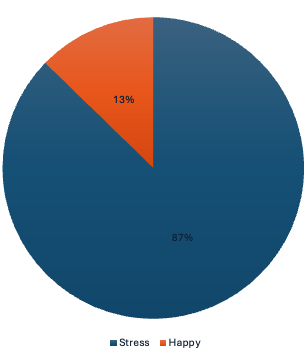
\includegraphics[width=0.45\linewidth]{image.png}
}
% \caption{Random Forest}
% \label{fig_ShaplyRF}
% \end{subfigure}
% \hfill
% \begin{subfigure}[t]{0.24\textwidth}
\subfloat[Trường hợp 2\label{feat_imb3}]{
    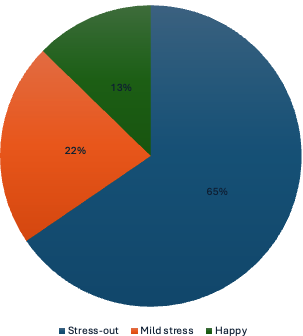
\includegraphics[width=0.45\linewidth]{3class.png}
}
% \caption{XGBoost model}
% \label{fig_ShaplyXG}
% \end{subfigure}
\caption{Sự mất cân bằng dữ liệu trong sự stress của sinh viên ở các trường hợp}
\label{feat_imb}
\end{figure}

\section{Cân bằng hoá dữ liệu}


% \subsection{Phương pháp truyền thống}

Trong nghiên cứu này, một sự kết hợp của các kỹ thuật tăng mẫu và giảm mẫu đã được sử dụng để nâng cao hiệu suất của mô hình phân loại và giải quyết sự mất cân bằng trong phân bố lớp học. Như được minh họa trong Phần \ref{relabel}, sự phân bố không đồng đều của dữ liệu trên các lớp là rõ ràng, với các lớp bị căng thẳng và bị căng thẳng quá mức chiếm hơn 85\% và 65\% dữ liệu huấn luyện trong hai trường hợp, cho thấy sự mất cân bằng đáng kể của dữ liệu stress. Để giảm thiểu vấn đề do sự mấy cân bằng này, sự kết hợp của kỹ thuật tăng mẫu thiểu số tổng hợp (SMOTE) \cite{SMOTE}, với liên kết Tomek \cite{T-links} (đối với trường hợp 2) và hàng xóm gần nhất được chỉnh sửa \cite{ENN} (đối với trường hợp 1) đã được sử dụng. Cách tiếp cận này giúp giảm bớt vấn đề mất cân bằng lớp học và thúc đẩy các dự đoán của mô hình chính xác và đáng tin cậy hơn.

% \subsection{Phương pháp dùng trí tuệ nhân tạo tạo sinh}
% (yet to be done, I have no idea how the model may afect final result, but will try SDV-Gausian Copulas, CopulasGAN, GAN, VAE)
\section{Mô hình huấn luyện}
Trong nghiên cứu này, tôi đã sử dụng ba mô hình học tập tổng hợp, cụ thể là Random Forest, XGBoost và SVM, để dự đoán mức độ căng thẳng hàng ngày bằng cách sử dụng tập đặc trưng đã trích xuất. Để đánh giá hiệu suất của các mô hình này, tôi đã sử dụng xác thực chéo (cross validation) 10 lần, một kỹ thuật được công nhận rộng rãi để đánh giá các thuật toán học máy.
\begin{itemize}
    \item Rừng ngẫu nhiên (RF) là một mô hình học tập, theo hệ số tạp chất Gini kết hợp các cây quyết định và quyết định dựa trên hệ số Gini. Kết quả của mô hình RF là trung bình của kết quả từ các cây quyết định bên trong nó. Nó tổng hợp kết quả từ nhiều cây quyết định để tạo ra một mô hình có độ lệch và phương sai thấp \cite{rf}.
    \item XGBoost là một thư viện tăng cường độ dốc phân tán được tối ưu hóa, được thiết kế để có hiệu quả cao, linh hoạt và di động \cite{xgb}. Nó triển khai các thuật toán học máy theo khung tăng cường độ dốc. XGBoost cung cấp một tăng cường cây song song (còn được gọi là GBDT, GBM) giải quyết nhiều vấn đề khoa học dữ liệu một cách nhanh chóng và chính xác. Cùng một mã chạy trên các môi trường phân tán chính (Hadoop, SGE, MPI) và có thể giải quyết các vấn đề vượt xa hàng tỷ ví dụ.
    \item Máy vectơ hỗ trợ (SVM) là một mô hình học máy cổ điển được thiết kế để tìm kiếm siêu mặt phẳng tối ưu để chia các lớp dữ liệu \cite{SVM}. Do đó, SVM đặc biệt hiệu quả cho các nhiệm vụ để phân biệt 2 hoặc nhiều lớp với độ chính xác cao.
\end{itemize}
Trong quá trình xác thực chéo, bộ dữ liệu được phân chia ngẫu nhiên thành mười tập con, với mỗi tập con đóng vai trò là tập kiểm tra một lần trong khi bốn tập con còn lại được sử dụng để huấn luyện. Quá trình này được lặp lại mười lần, đảm bảo rằng mỗi tập con được sử dụng chính xác một lần làm tập kiểm tra.

Hơn nữa, để đảm bảo tính mạnh mẽ của các đánh giá mô hình của tôi, việc chia tách huấn luyện-kiểm tra được tiến hành ngẫu nhiên giữa tất cả các tình nguyện viên nghiên cứu. Cách tiếp cận này cho phép tôi đánh giá khả năng chung và hiệu quả của các mô hình dự đoán của tôi trên các cá nhân khác nhau trong nhóm tình nguyện viên.

Để đánh giá hiệu suất phân loại của các mô hình của tôi, tôi đã sử dụng mười số liệu đánh giá: độ chính xác, điểm F1 của lớp căng thẳng cao, điểm Weighted F1 và điểm Macro F1. 
Về các số liệu đánh giá, chúng cho phép đánh giá toàn diện hiệu suất của mô hình, xem xét các khía cạnh khác nhau như độ chính xác tổng thể, độ chính xác, độ nhạy và điểm F1, cung cấp một sự hiểu biết sắc thái về hiệu quả của mô hình trong việc phân loại mức độ căng thẳng. Những phân tích thống kê này tạo điều kiện cho việc đánh giá kỹ lưỡng các mô hình của tôi, cho phép tôi đánh giá hiệu quả của chúng và xác định các lĩnh vực cần cải thiện.

\section{Phương pháp đánh giá mô hình}
% Một trong những đánh giá phổ biến trong học máy là báo cáo mô hình phân loại. Trong báo cáo này các đặc trưng (\ref{acc}-\ref{Weighted}) sẽ được sử dụng:
\begin{equation}
    Precision=\frac{TP}{TP+FP}
    \label{P}
\end{equation}
\begin{equation}
    Recall=\frac{TP}{TP+FN}
    \label{R}
\end{equation}
\begin{equation}
    Accuracy=\frac{TP+TN}{TP+TN+FN+FP}
    \label{acc}
\end{equation}
\begin{equation}
    F1=\frac{2\times Precision \times Recall}{Precision+Recall}
    \label{F1}
\end{equation}
\begin{equation}
    Weighted\_F1=\frac{\sum{n_i\times F1_i}}{\sum{n_i}}
    \label{Weighted}
\end{equation}
\begin{equation}
    Macro\_F1=\frac{\sum{F1_i}}{\sum{class}}
    \label{MacroF1}
\end{equation}
với
\begin{itemize}
    \item TP, FP, FN, TN được đề cập trong hình \ref{confmat_img}
    \item $n_i$ là số lượng mẫu hỗ trợ lớp i
    \item $F1_i$ là hệ số F1 (xem công thức \eqref{F1}) của lớp i
\end{itemize} 

\begin{figure}[ht]
    \centering
    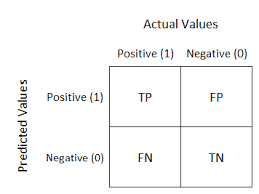
\includegraphics[width=0.5\linewidth]{images-5.png}
    \caption{Hình ảnh trực quan các giá trị trong ma trận nhầm lẫn}
    \label{confmat_img}
\end{figure}

Trong học máy, để đánh giá hiệu suất của một mô hình, độ chính xác \eqref{acc} (accuracy) được sử dụng phổ biến. Giá trị này thể hiện tỷ lệ các dự đoán đúng so với tổng số dự đoán. Độ chính xác thường được chọn làm thước đo đầu tiên bởi tính đơn giản, trực quan và dễ tính toán của nó. Nó cung cấp một cái nhìn tổng quan về hiệu suất chung của mô hình, giúp các nhà nghiên cứu và kỹ sư có thể so sánh hiệu quả giữa các mô hình khác nhau.

Mặc dù vậy, độ chính xác lại có những hạn chế nhất định khi áp dụng cho các tập dữ liệu không cân bằng. Trong trường hợp này, một mô hình có thể đạt được độ chính xác cao đơn giản bằng cách dự đoán tất cả các mẫu vào lớp chiếm đa số. Để khắc phục vấn đề này, các nhà nghiên cứu đã đề xuất sử dụng các thước đo khác, điển hình là weighted F1-score.

Weighted F1-score \eqref{Weighted} là một thước đo tổng hợp, kết hợp cả precision (độ chính xác \eqref{P}) và recall (độ phủ \eqref{R}). Nó tính toán trung bình hài hòa có trọng số của precision và recall, trong đó trọng số của mỗi lớp được điều chỉnh để phản ánh tầm quan trọng tương đối của chúng. Nhờ vậy, weighted F1-score cung cấp một cái nhìn toàn diện hơn về hiệu suất của mô hình, đặc biệt trong các bài toán phân loại có dữ liệu không cân bằng. Việc sử dụng weighted F1-score giúp đảm bảo rằng mô hình không chỉ tập trung vào việc dự đoán chính xác lớp chiếm đa số mà còn chú trọng đến việc phân loại chính xác các lớp thiểu số.

Do những lý do nêu trên, độ chính xác, F1 score lớp stress, và F1 có trọng số sẽ được sử dụng ở bài luận này để đánh giá độ hiệu quả của mô hình.

\section{Phân tích đặc trưng thông qua hệ thống trí tuệ nhân tạo giải thích}
% \subsection{SHAP}
Để hiểu cách mô hình và các đặc trưng đã trích xuất hoạt động, các giá trị SHAPley (SHapley Additive exPlanations) - một công cụ mạnh mẽ để biết được các lý do quyết định của mô hình bằng cách sử dụng lý thuyết trò chơi làm cơ sở để đo lường sự đóng góp của mỗi yếu tố vào mô hình học máy. Nghiên cứu này sử dụng TreeExplainer của khung SHAP để tính toán các giá trị SHAPley (giá trị SHAP) nhanh hơn \cite{tree_explainer} .

Giá trị Shapley là một công cụ mạnh mẽ để đo lường sự đóng góp công bằng của từng người chơi trong một trò chơi hợp tác\cite{shap_value}. Giá trị SHAPley ($\phi_i(x)$) được định nghĩa bởi: 
\begin{equation}
  \phi _i (x) = \sum _{S \subseteq F \setminus \{i\}} \frac{|S|!(|F|-|S|-1)!}{|F|!}[f_{S \cup \{i\}}(x_{S \cup \{i\}})-f_{S }(x_{S })]
\end{equation}  
với:
 \begin{itemize}
   \item $x$: đối tượng quan sát 
   \item $F$: tổng đặc trưng
   \item $f_S$: mô hình huấn luyện trên đặc trưng S
   
   \item $f_{S \cup \{i\}}$: mô hình huấn luyện trên đặc trưng S và i
  \item $x_S$: giới hạn đối tượng quan sát trên miền đặc trưng S
  \item $x_{S \cup \{i\}}$: giới hạn đối tượng quan sát trên miền đặc trưng S và i
 \end{itemize}

Trong lĩnh vực học máy, các đặc trưng đóng vai trò là những người chơi chính quyết định kết quả của mô hình dự đoán, tương tự như những người tham gia trong một trò chơi. Sử dụng các giá trị SHAPley, sự đóng góp của mỗi đặc trưng vào đầu ra của mô hình được làm rõ thông qua các loại biểu đồ khác nhau, hỗ trợ trong việc giải thích hành vi của mô hình.

Một trong những hình ảnh trực quan như vậy, biểu đồ phân tán mật độ, mô tả các giá trị SHAP của mỗi đặc trưng trên tất cả các trường hợp trong tập kiểm tra. Biểu đồ phân tán này cho phép hiểu rõ cách mỗi đặc trưng ảnh hưởng đến các dự đoán của mô hình trên các trường hợp khác nhau. Bằng cách kiểm tra sự phân bố của các giá trị SHAP, chúng ta có thể nhận ra tác động của từng đặc trưng đối với kết quả của mô hình đối với các trường hợp kiểm tra khác nhau.
% \subsection{LIME}
% Một mô hình XAI khác có thể kể tới là LIME \cite{LIME} (Local Interpretable Model-Agnostic Explanations). Với LIME, các yếu tố được quan sát một cách cục bộ, từ đó ta có cái nhìn chi tiết hơn về từng thành phần của mẫu so với SHAP. Và với cái nhìn về từng cá thể của LIME, ta có thể làm bật nên những điểm dữ liệu có tính đặc biệt.

% Về cách thức hoạt động, LIME dựa trên sự biến đổi nhỏ của dữ liệu gốc. Chi tiết hơn, LIME sẽ tạo những phiên bản có sự xê dịch của dữ liệu gốc, sau đó sẽ cho dữ liệu bị xê dịch này vào trong mô hình học máy cần giải thích. Với các xê dịch này sẽ tạo những tạo nên những thay đổi cục bộ mà LIME sẽ dùng để giải thích trên các đặc trưng. Sau đó LIME sẽ đo sức nặng của các yếu tố đặc trưng cục bộ này và sau đó sẽ đưa ra được các giải thích cho từng mẫu quan sát. 